\begin{frame}
\frametitle{Alice is surfing...}
  \begin{block}{}
    \vskip -1.2cm
    \begin{figure}[t]
    \centering
     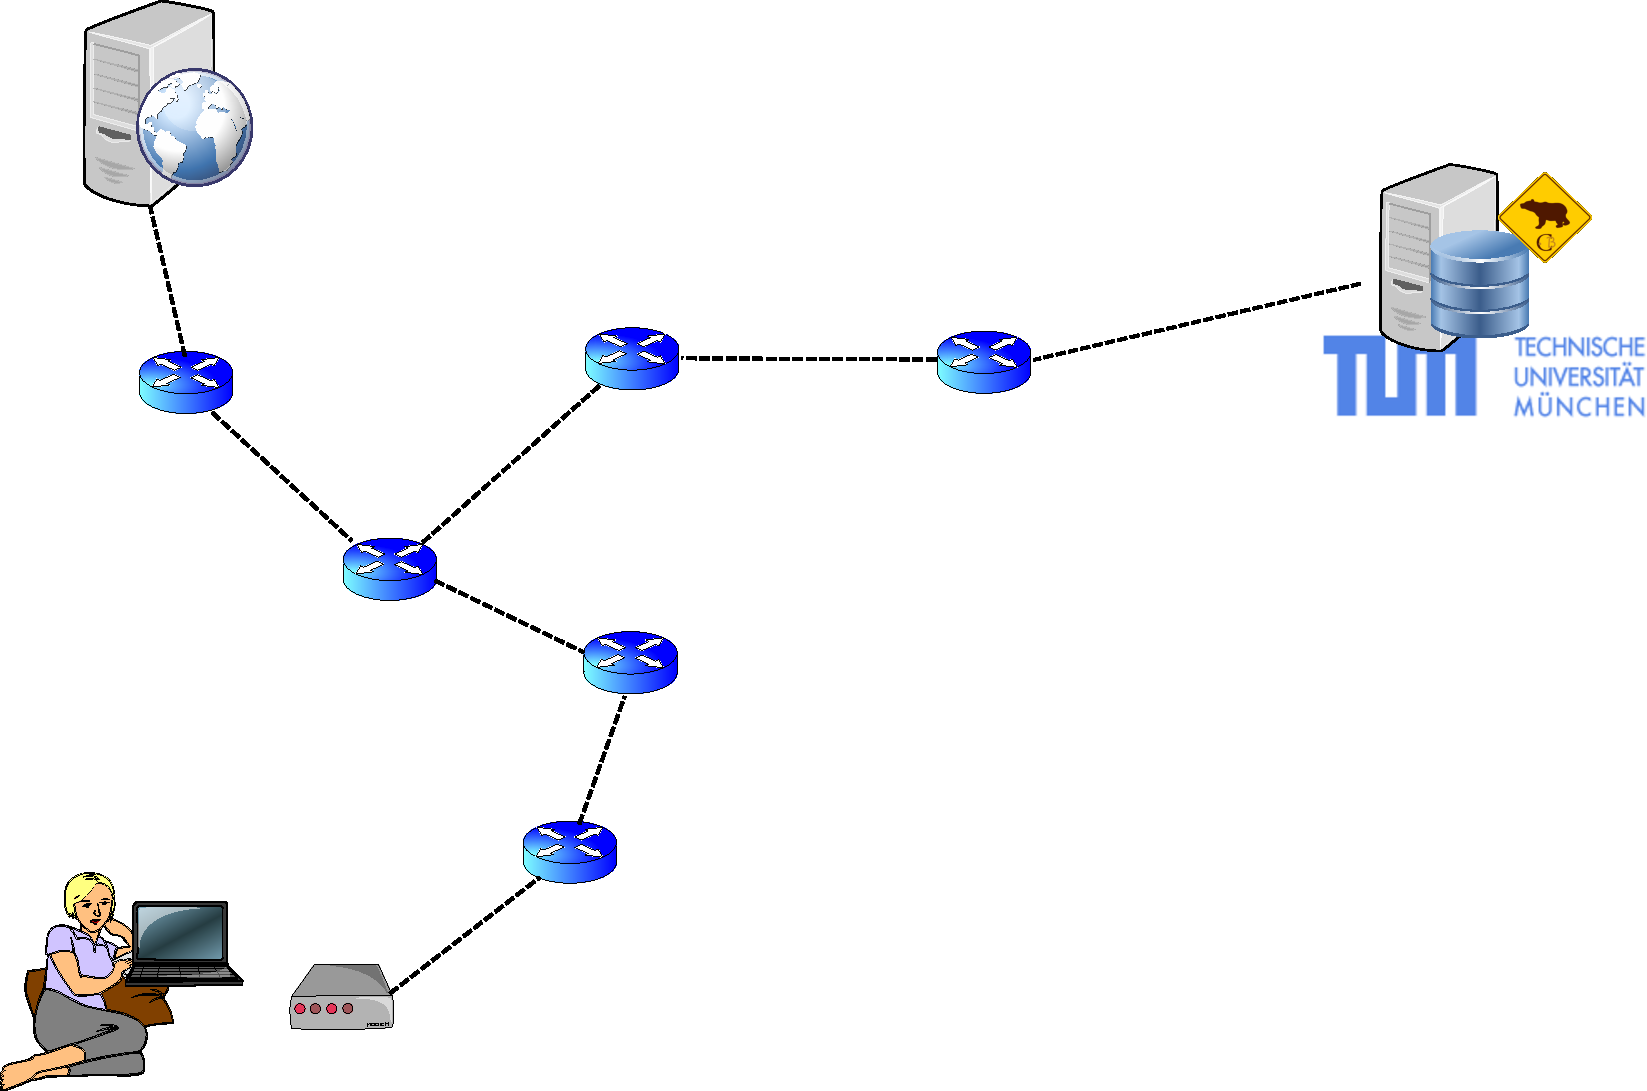
\includegraphics[scale=.36]{figures/reporting}
    \end{figure}
  \end{block}
\end{frame}

\begin{frame}
\frametitle{Man-in-the-middle}
  \begin{block}{}
    \vskip -1.1cm
    \begin{figure}[t]
    \centering
     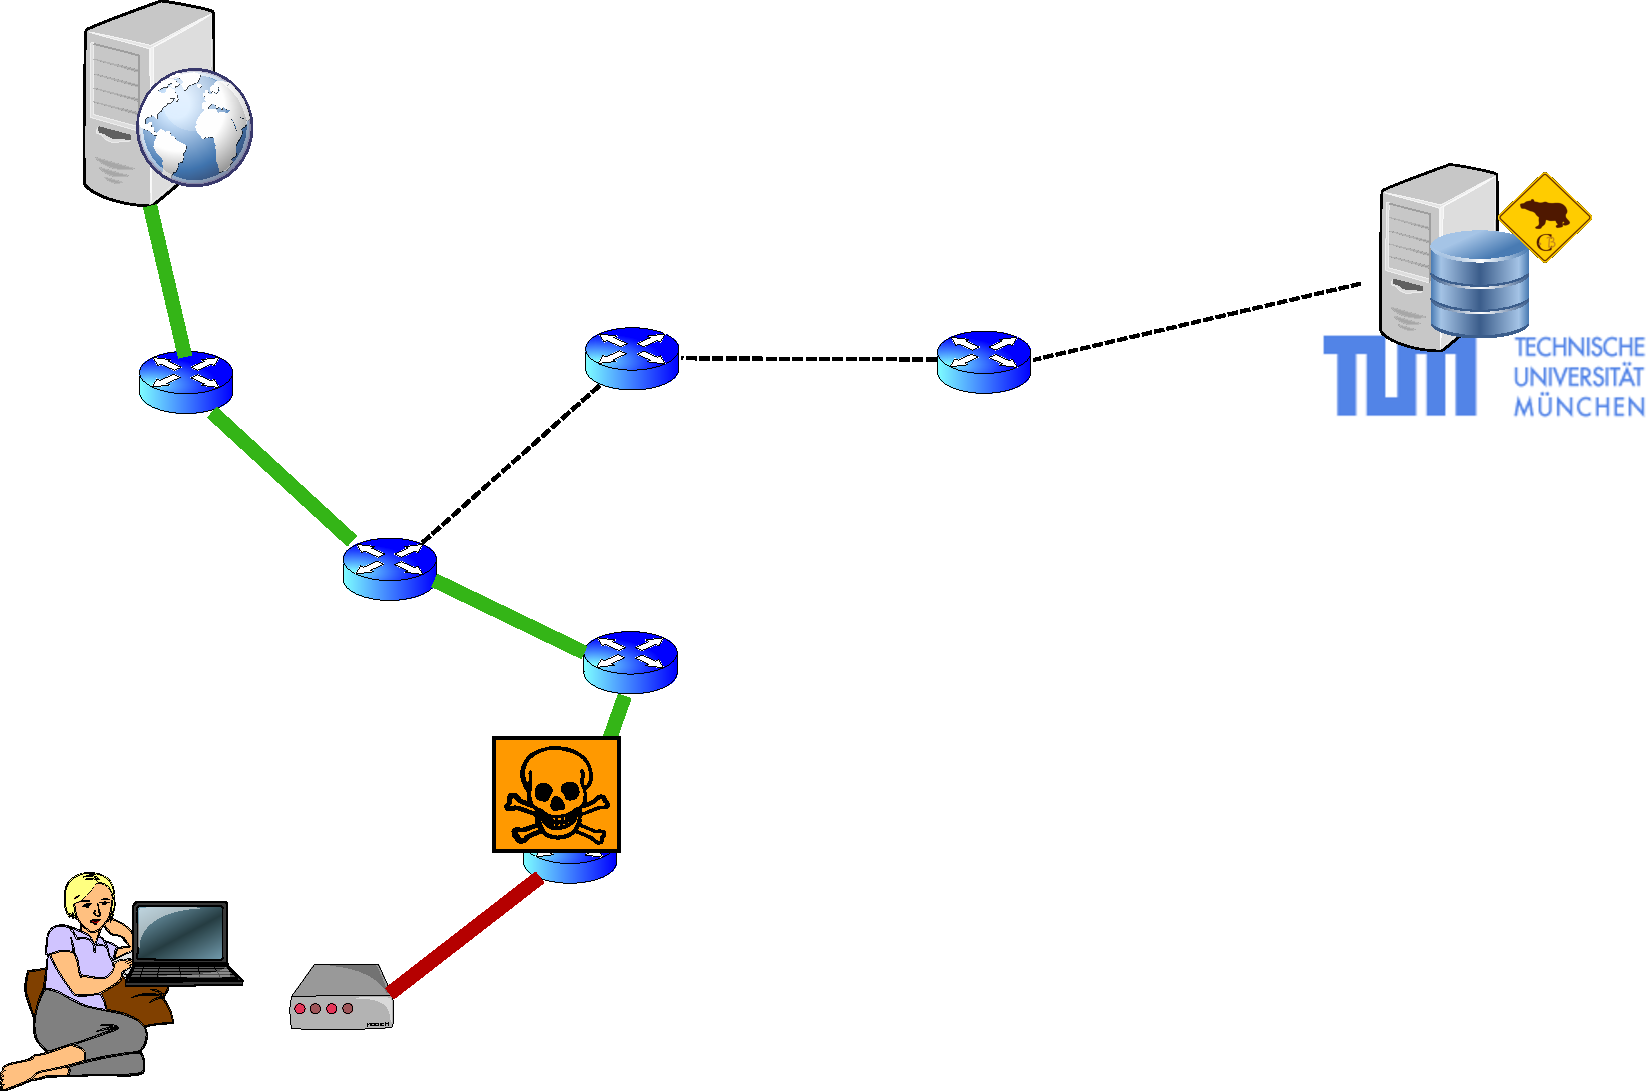
\includegraphics[scale=.36]{figures/reporting-2-attacked}
    \end{figure}
  \end{block}
\end{frame}

\begin{frame}
\frametitle{Alice queries Crossbear}
  \begin{block}{}
    \vskip -1.2cm
    \begin{figure}[t]
    \centering
     \includegraphics[scale=.36]{figures/reporting-3-querying}
    \end{figure}
  \end{block}
\vskip -.5cm
\begin{block}{\small NB: SSL-secured connection, server cert hard-coded}\end{block}
\end{frame}

\begin{frame}
\frametitle{Crossbear checks the server}
  \begin{block}{}
    \vskip -1.1cm
    \begin{figure}[t]
    \centering
     \includegraphics[scale=.36]{figures/reporting-4-checking}
    \end{figure}
  \end{block}
\end{frame}


\begin{frame}
\frametitle{Crossbear reports result}
  \begin{block}{}
    \vskip -1.2cm
    \begin{figure}[t]
    \centering
     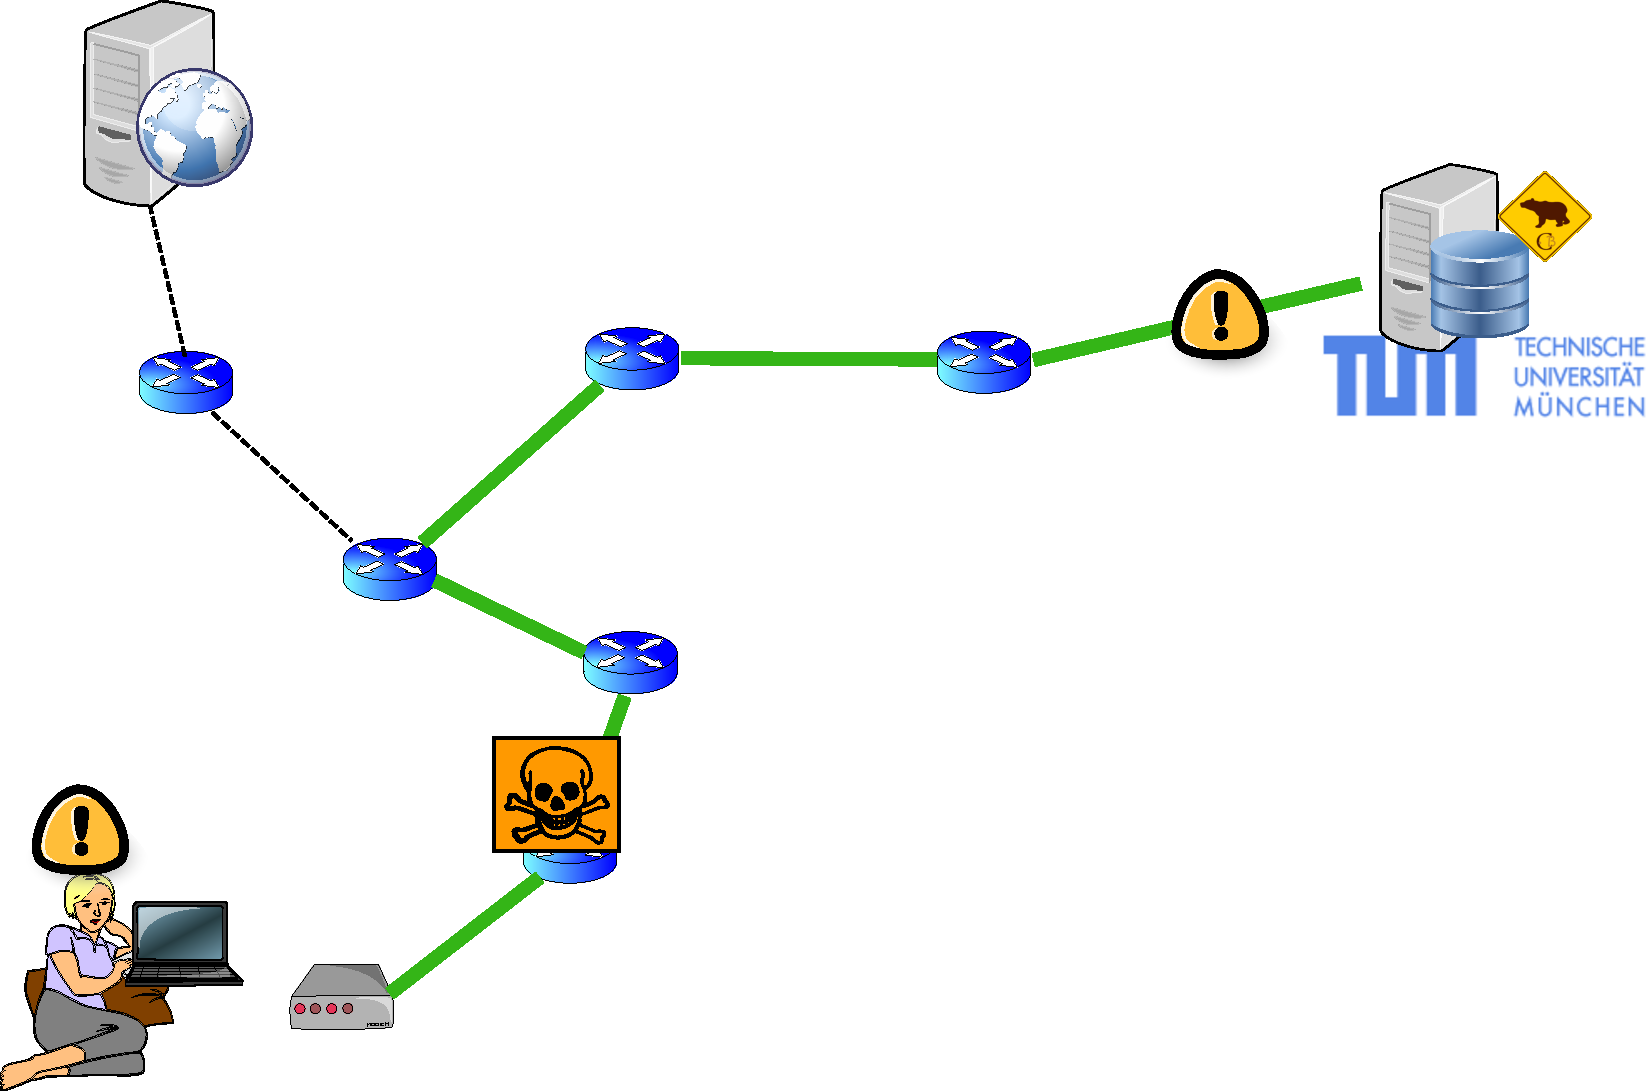
\includegraphics[scale=.36]{figures/reporting-5-feedback}
    \end{figure}
  \end{block}
\end{frame}


\begin{frame}
\frametitle{Alice traceroutes to server}
  \begin{block}{}
    \vskip -1.1cm
    \begin{figure}[t]
    \centering
     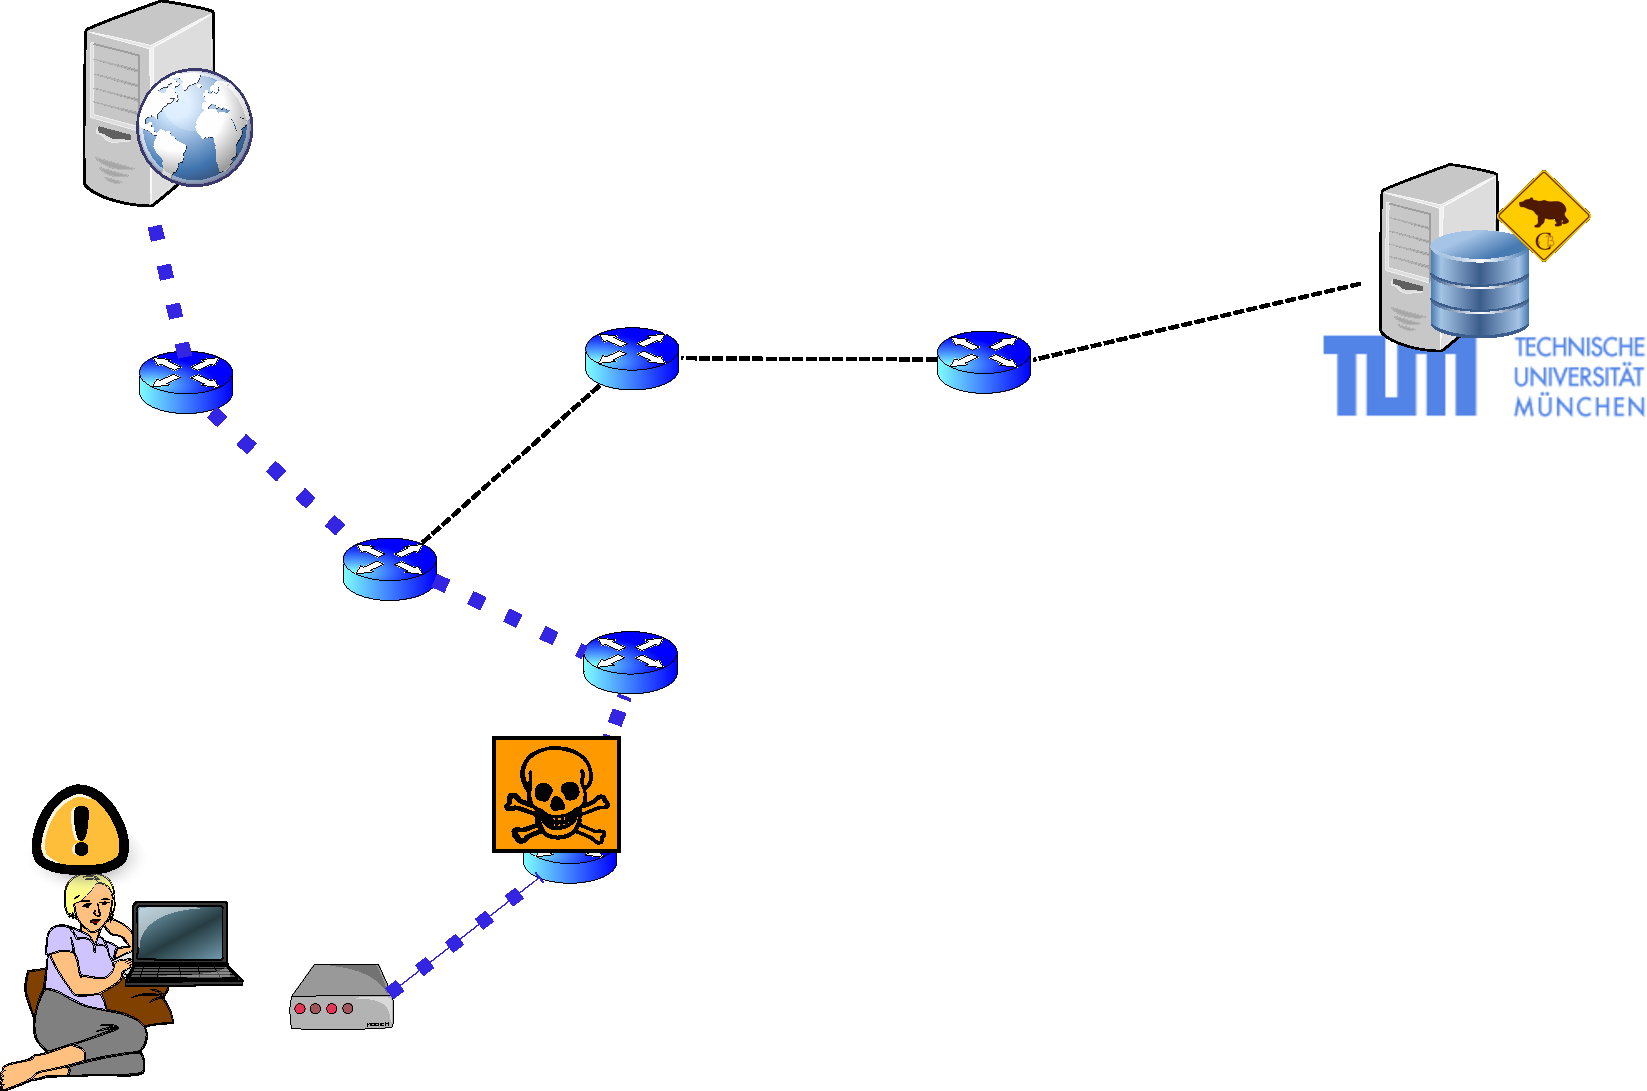
\includegraphics[scale=.36]{figures/reporting-6-hunting}
    \end{figure}
  \end{block}
\end{frame}


\begin{frame}
\frametitle{Alice reports to Crossbear}
  \begin{block}{}
    \vskip -1.2cm
    \begin{figure}[t]
    \centering
     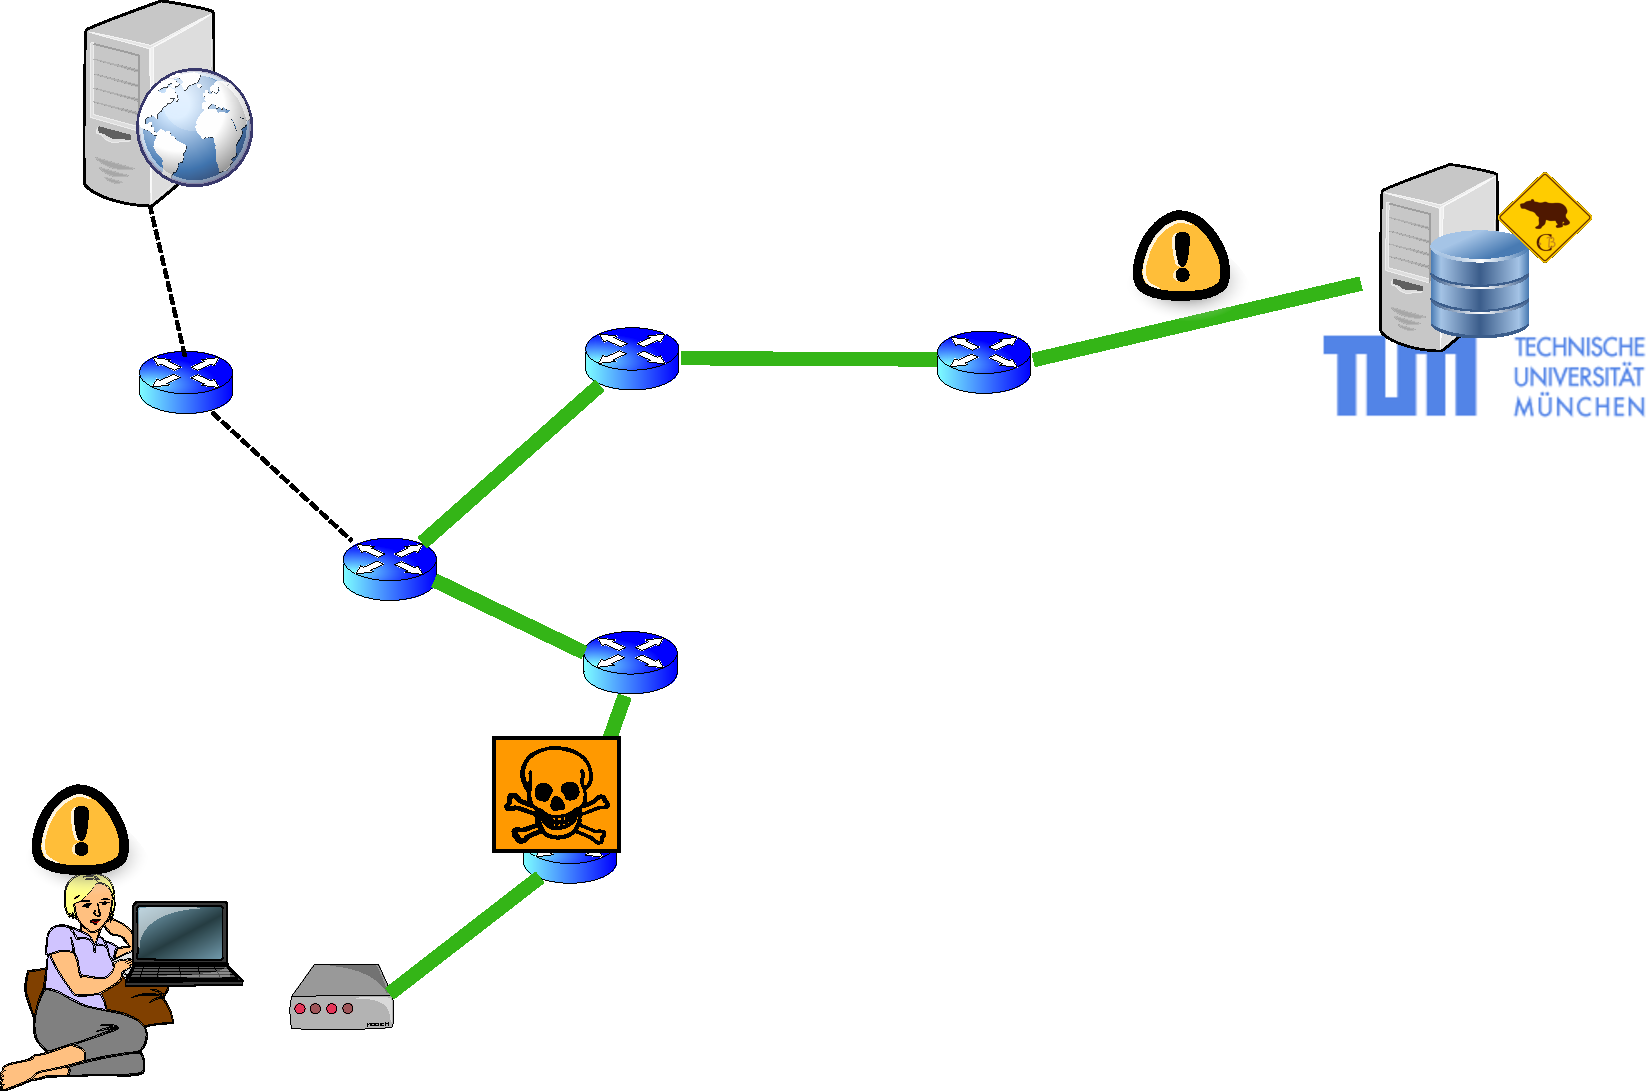
\includegraphics[scale=.36]{figures/reporting-7-huntingreport}
    \end{figure}
  \end{block}
\end{frame}

\begin{frame}
\frametitle{Distribute hunting tasks}
  \begin{block}{}
    \vskip -1.2cm
    \begin{figure}[t]
    \centering
     \includegraphics[scale=.36]{figures/hunting-1-polling}
    \end{figure}
  \end{block}
\end{frame}

\begin{frame}
\frametitle{Bob goes hunting}
  \begin{block}{}
    \vskip -1.2cm
    \begin{figure}[t]
    \centering
     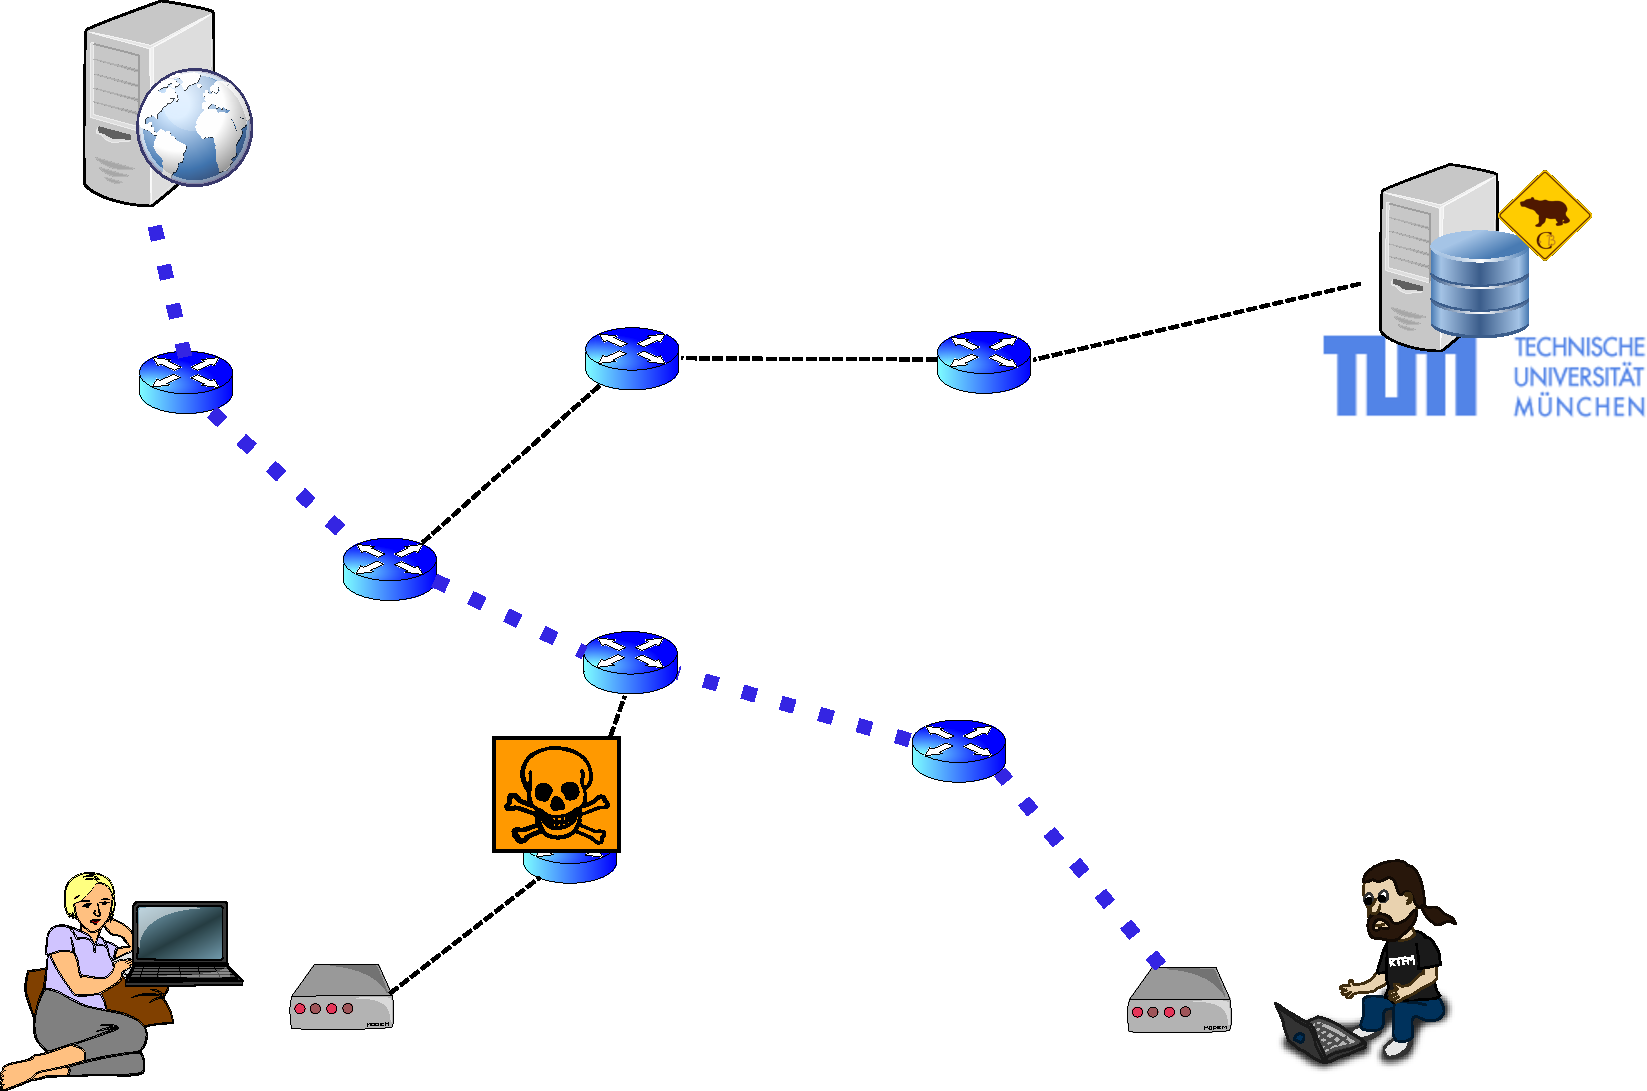
\includegraphics[scale=.36]{figures/hunting-2-hunting}
    \end{figure}
  \end{block}
\end{frame}

\begin{frame}
\frametitle{Bob reports}
  \begin{block}{}
    \vskip -1.2cm
    \begin{figure}[t]
    \centering
     \includegraphics[scale=.36]{figures/hunting-3-reporting}
    \end{figure}
  \end{block}
\end{frame}

\begin{frame}
\frametitle{There are many Bobs}
  \begin{block}{}
    \vskip -1.2cm
    \begin{figure}[t]
    \centering
     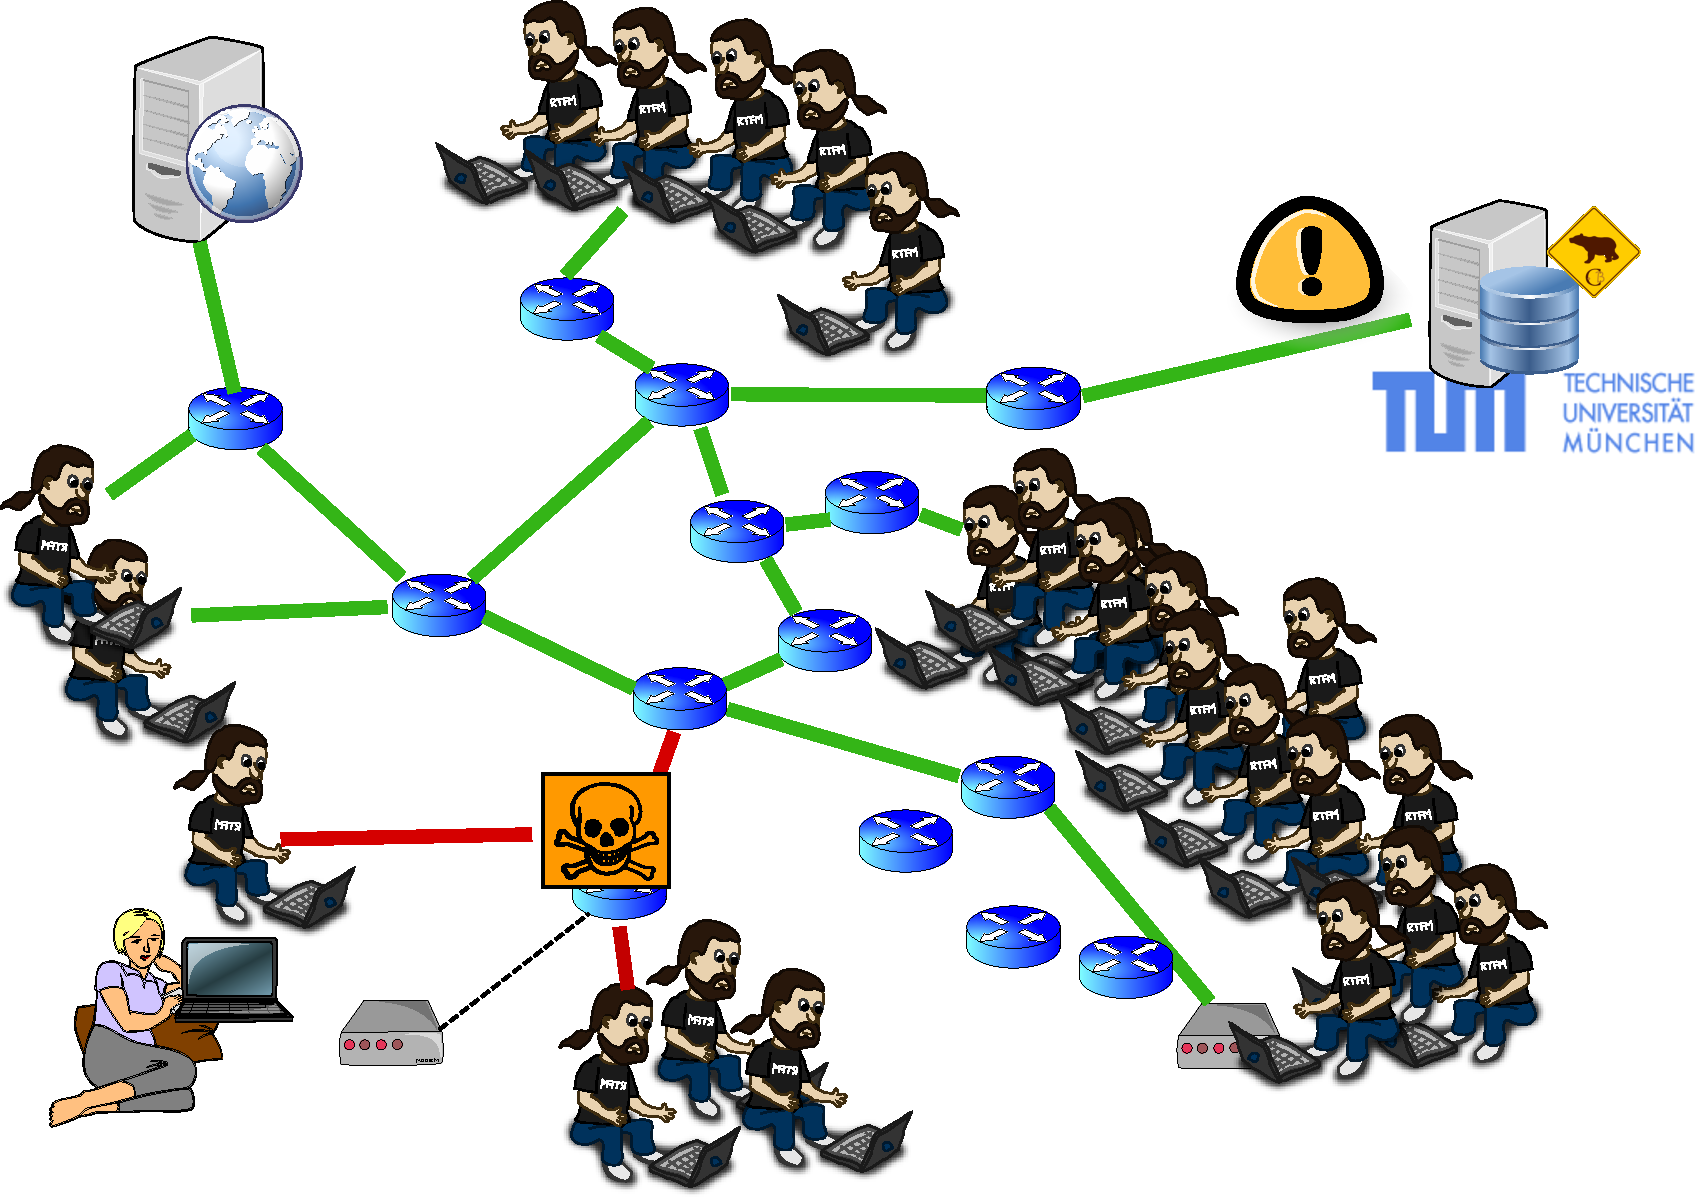
\includegraphics[scale=.36]{figures/hunting-4-manyreporting}
    \end{figure}
  \end{block}
\end{frame}


%\begin{frame}
%\frametitle{Components}
%\begin{block}{Server: store and analyse}
%  \begin{itemize}
%    \item Crossbear server at TU M{\"u}nchen, Germany
%    \item Uses Convergence project's notaries for diversity
%    \item Server cert hard-coded into client!
%  \end{itemize}
%\end{block}
%\begin{block}{Detection and localisation}
%  \begin{itemize}
%    \item Clients as Firefox add-on (detection and localisation)
%    \item 150 stand-alone hunters on stand-by on PlanetLab (localisation)
%  \end{itemize}
%\end{block}
%\end{frame}




\begin{frame}
\frametitle{Additional data raised}
\begin{block}{Actually, we also determine on server-side:}
  \begin{itemize}
    \item CAs used in certificate chain ($\rightarrow$ continuity)
    \item AS number of hosts in traceroute \\ ($\rightarrow$ frequent reports?)
    \item Geo data: location of hosts in traceroute \\ ($\rightarrow$ traversed countries)
    \item WHOIS info
  \end{itemize}
\end{block}
\begin{block}{Firefox add-on for \textit{detection} and \textit{hunting}}
  \begin{itemize}
    \item For \textit{savvy users}
    \item Score-based, several factors
    \item UI $\rightarrow$ see code on github
  \end{itemize}
\end{block}
\end{frame}


\begin{frame}
\frametitle{TODO: Integration into OONI}
\begin{block}{OONI is for hunting}
  \begin{itemize}
    \item Arguments for OONI
    \item MITM testing ground
    \item What data is sent (privacy?)
    \item Visualisation mock-up
    \item If OONI had been active during the Iran MITM... what would we have found?
  \end{itemize}
\end{block}
\end{frame}

%\begin{frame}
%\frametitle{Attacker model}
%\begin{block}{Chosen based on MitM reports we have}\end{block}
%\begin{block}{Attacker behaviour}
%  \begin{itemize}
%    \item Non-selective: MitM all attached `client' systems
%    \item Selective: MitM only some of attached `client' systems
%  \end{itemize}
%\end{block}
%\begin{block}{Attacker position}
%  \begin{itemize}
%    \item Towards periphery, close to victim client
%    \item Towards periphery, close to victim server
%    \item Central location in network (important AS, ...)
%  \end{itemize}
%\end{block}
%\end{frame}


\begin{frame}
\frametitle{Non-selective, close to victim client}
\begin{block}{}
  \begin{figure}[t]
    \centering
    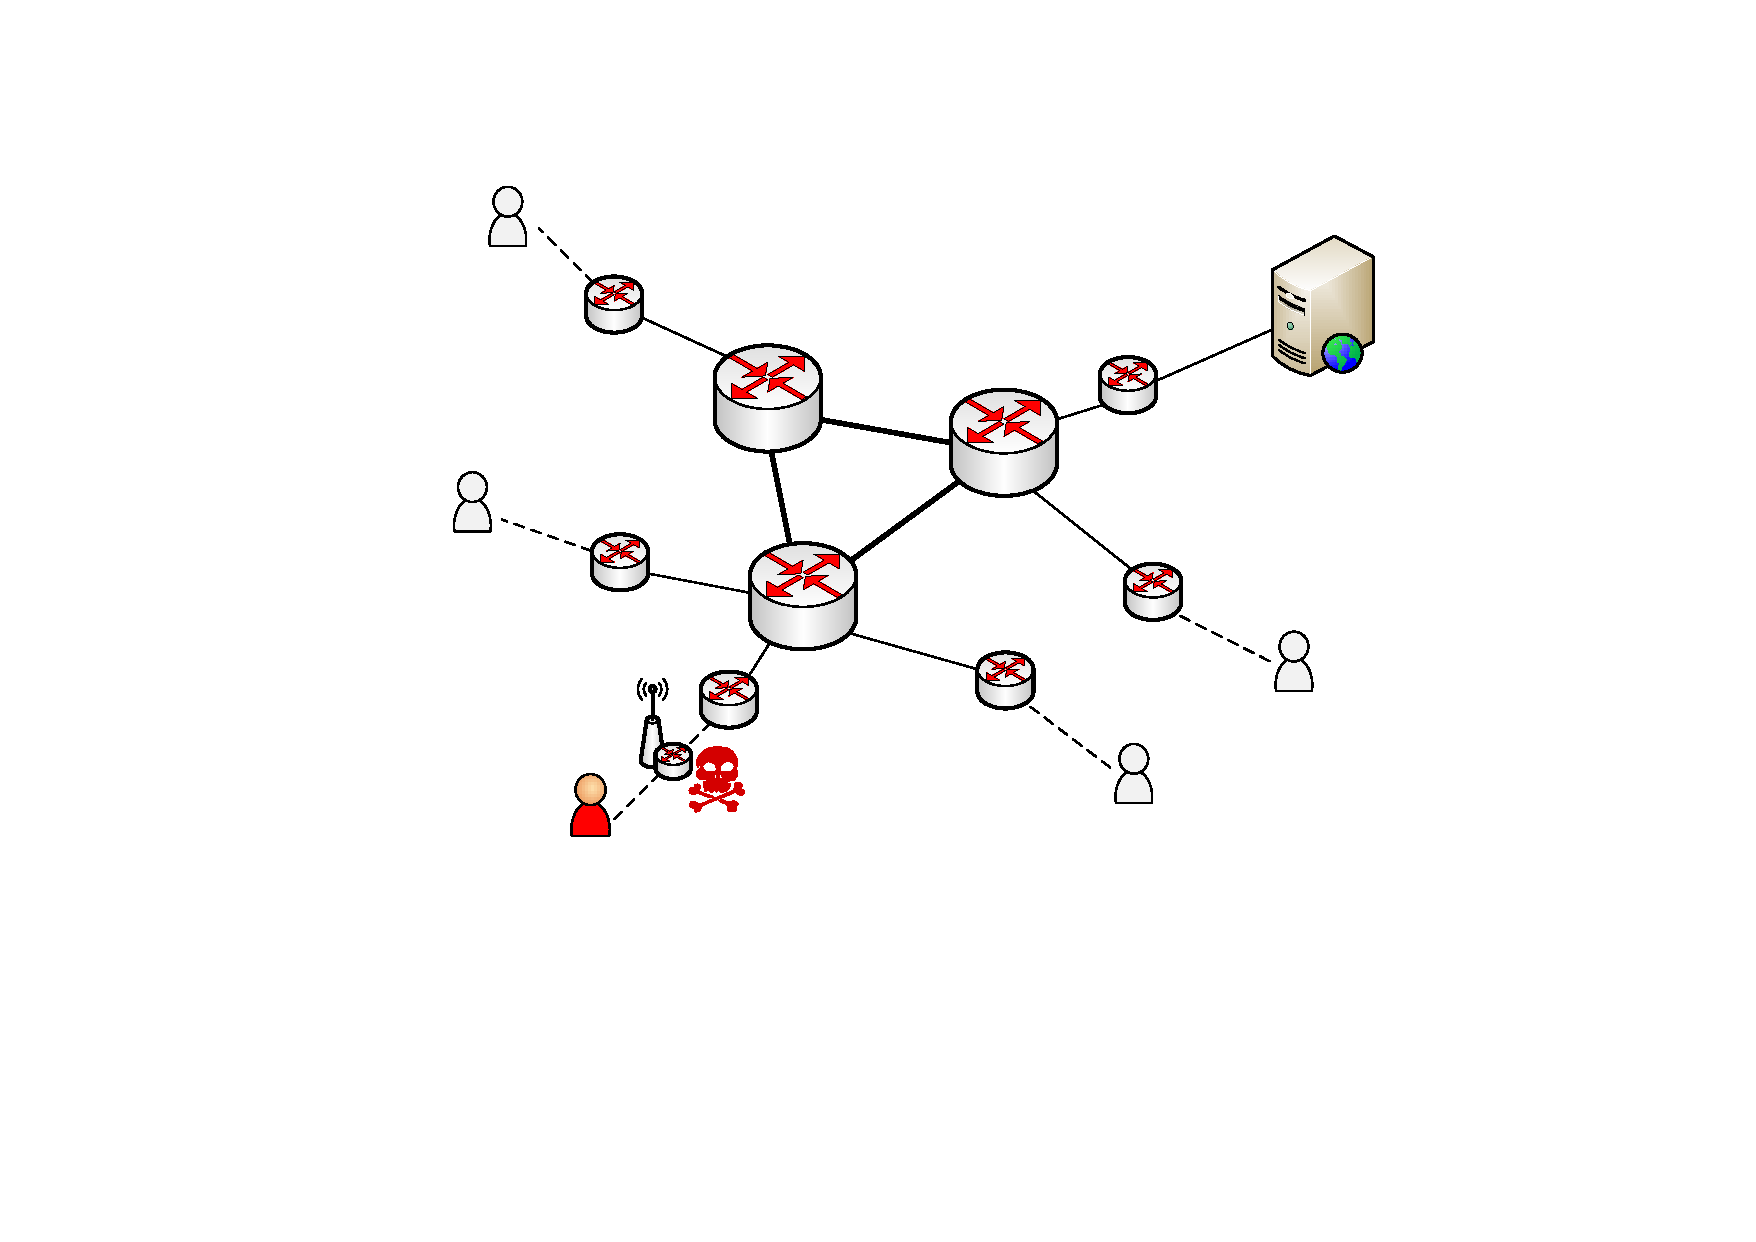
\includegraphics[scale=.5]{figures/scenario1-close-to-ap.pdf}
  \end{figure}
\end{block}
\end{frame}



\begin{frame}
\frametitle{Non-selective, state-level attacker}
\begin{block}{}
  \begin{figure}[t]
    \centering
    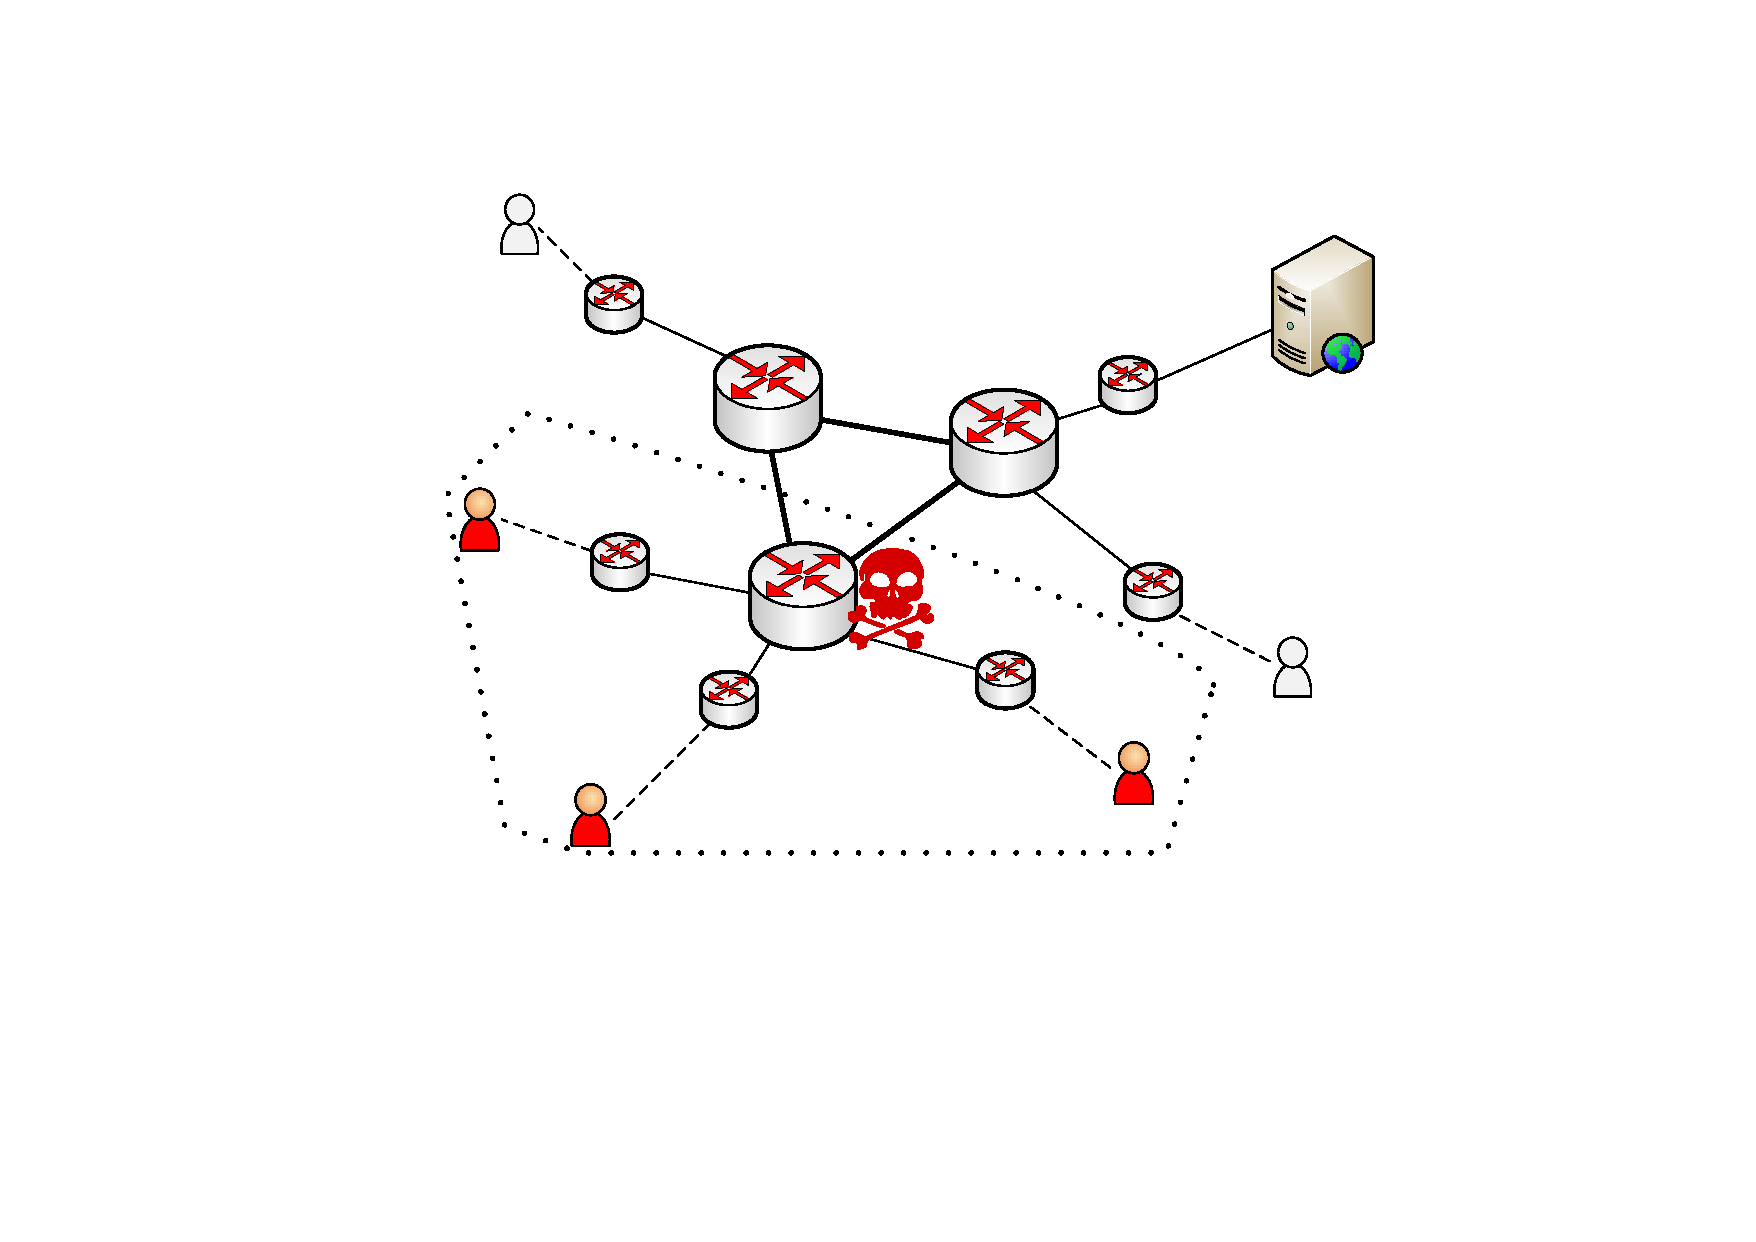
\includegraphics[scale=.5]{figures/scenario5-stateattacker-non-selective.pdf}
  \end{figure}
\end{block}
\end{frame}




\begin{frame}
\frametitle{Analysis: non-selective attacker}
\begin{block}{Detection}
  \begin{itemize}
    \item Attack is detected if $\geq 1$ reports
%    \item Attacker can only drop connections to Crossbear server
  \end{itemize}
\end{block}
\begin{block}{Lends itself well to localisation}
  \begin{itemize}
    \item Get $\geq 1$ traceroute from victim,  $\geq 1$ from unpoisoned hunter 
    \item The more, the better. The closer to intersection point, the better.
%    \item Success depends on the number of hunters
    \item An estimate can be given: \\ $<100$ hunters for $95\%$ accuracy on AS-level
    \item Adaptive attackers are a problem (can't discuss here)
    \item Full details in our research paper
  \end{itemize}
\end{block}
\end{frame}



%\begin{frame}
%\frametitle{Number of hunters vs. success}
%\vskip -.7cm
%\begin{block}{}
%  \begin{figure}[t]
%    \centering
%    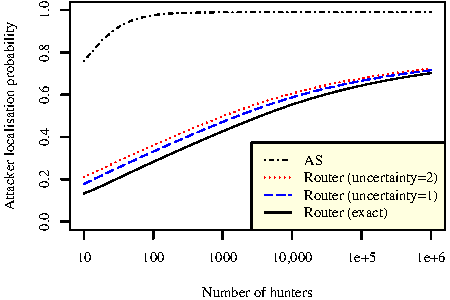
\includegraphics[scale=1.2]{figures/plot.pdf}
%  \end{figure}
%\end{block}
%\begin{block}{Imperfect, but given lack of data probably the best we can get.}\end{block}
%\end{frame}


\begin{frame}
\frametitle{Different problem: SSH}
\begin{figure}[t]
  \centering
  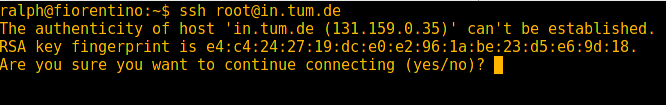
\includegraphics[scale=.65]{figures/ssh-connect.png}
\end{figure}
\begin{block}{Ever had this problem?}
\begin{itemize}
  \item Want to compare an SSH fingerprint without 2nd channel?
  \item No idea what the correct host-key should be?
\end{itemize}
\end{block}
\end{frame}







%\begin{frame}
%\frametitle{What's next?}
%  \begin{block}{Integration with OONI}
%    \begin{itemize}
%      \item Open Observatory of Network Interference
%      \item Hopefully, many clients soon
%      \item Plus people who are in the right locations...
%      \item That is where all our efforts will go into in the next 6 months
%    \end{itemize}
%  \end{block}
%  \begin{block}{Analysis tools}
%    \begin{itemize}
%      \item Automate analysis of reports
%      \item Filter out and group by suspicious cases
%    \end{itemize}
%  \end{block}
%\end{frame}


\begin{frame}
\frametitle{Thank you!}
\vskip 1cm
  \begin{center}
    
\includegraphics[scale=0.2]{figures/question_mark.pdf}
  \end{center}
\begin{block}{Contact}
      \begin{itemize}
	\item Twitter: @crossbearteam
        \item WWW: \texttt{https://pki.net.in.tum.de}
        \item \url{https://github.com/crossbear/Crossbear}
      \end{itemize}
  \end{block}
\end{frame}



\begin{frame}
\frametitle{Selective attacker: close to victim}
\begin{block}{}
  \begin{figure}[t]
    \centering
    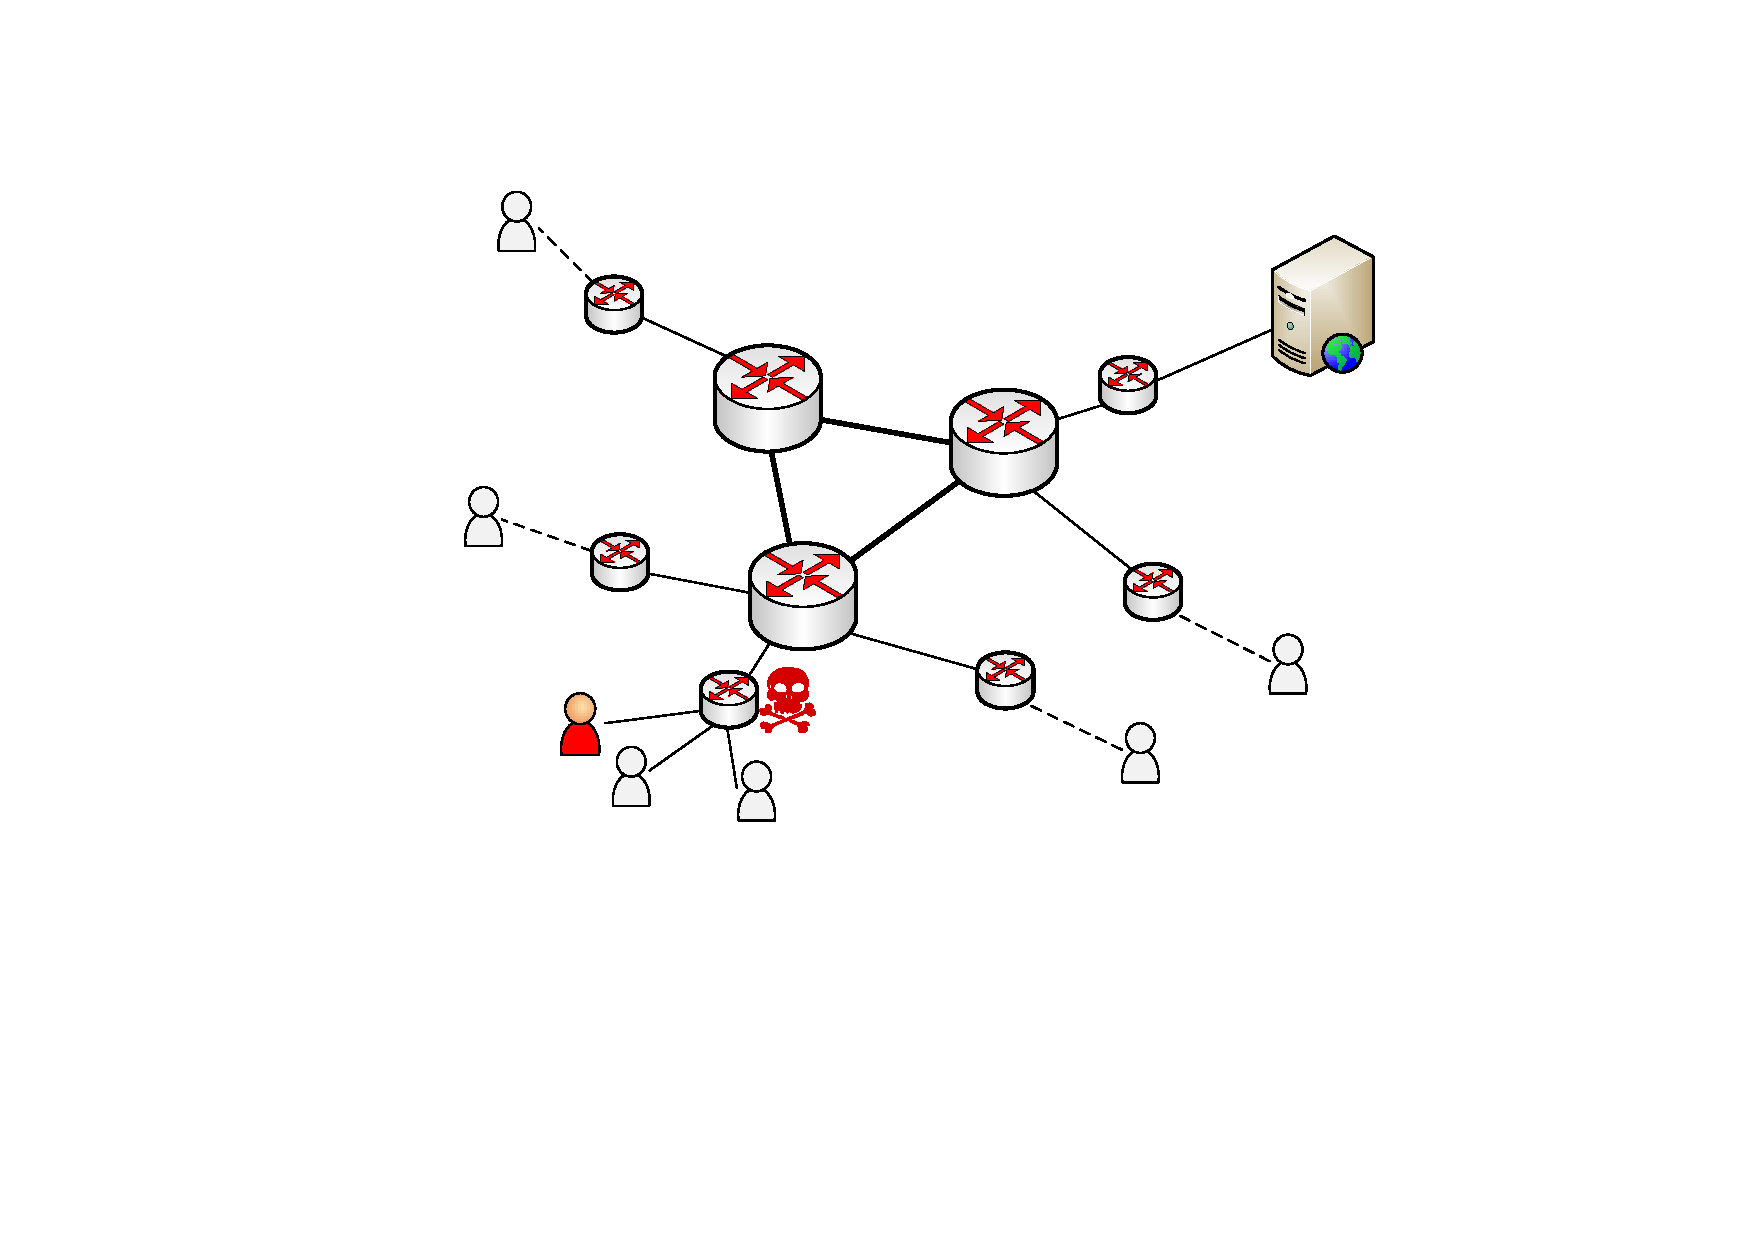
\includegraphics[scale=.5]{figures/scenario3-close-to-ap-selective.pdf}
  \end{figure}
\end{block}
\end{frame}

\begin{frame}
\frametitle{Selective attacker: in core}
\begin{block}{}
  \begin{figure}[t]
    \centering
    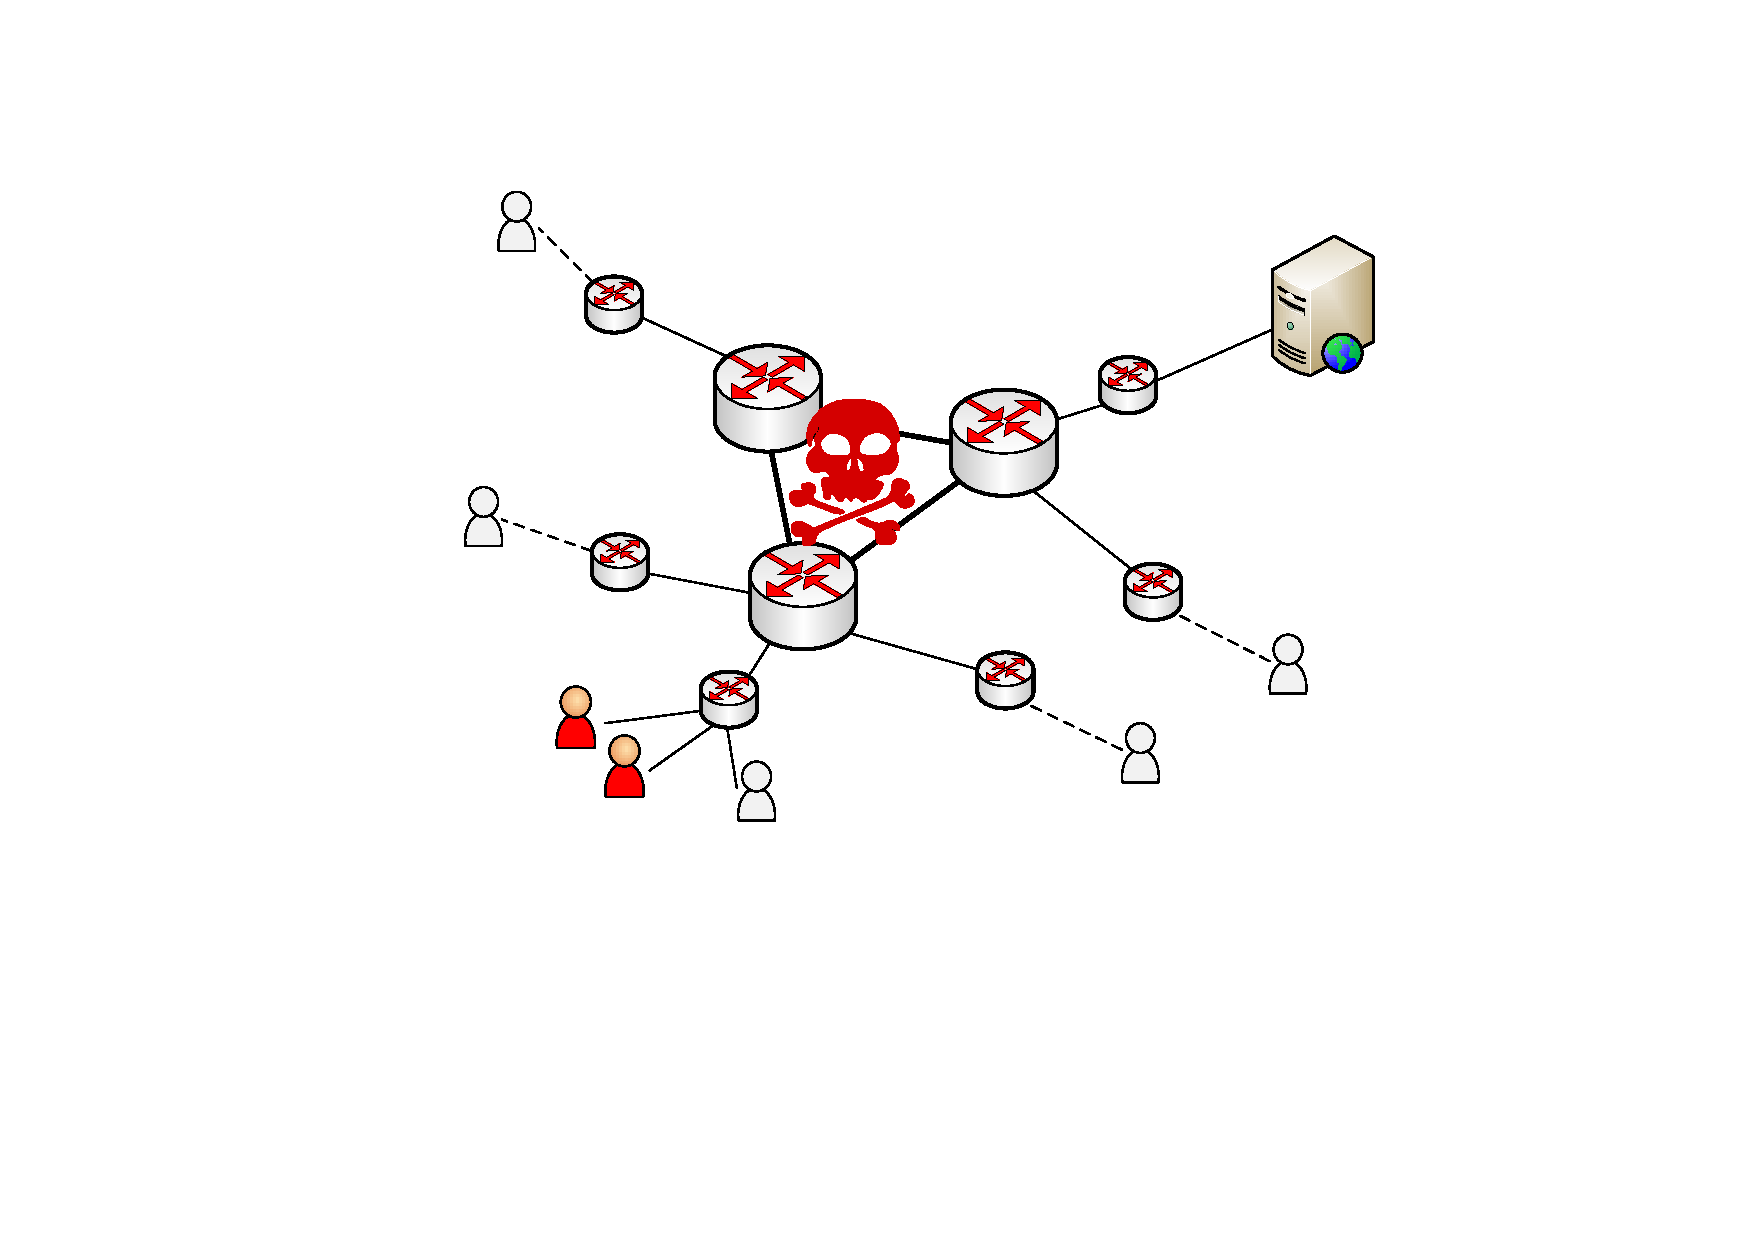
\includegraphics[scale=.5]{figures/scenario4-core-selective.pdf}
  \end{figure}
\end{block}
\end{frame}



\begin{frame}
\frametitle{Selective attackers are a headache}
  \begin{figure}[t]
    \centering
    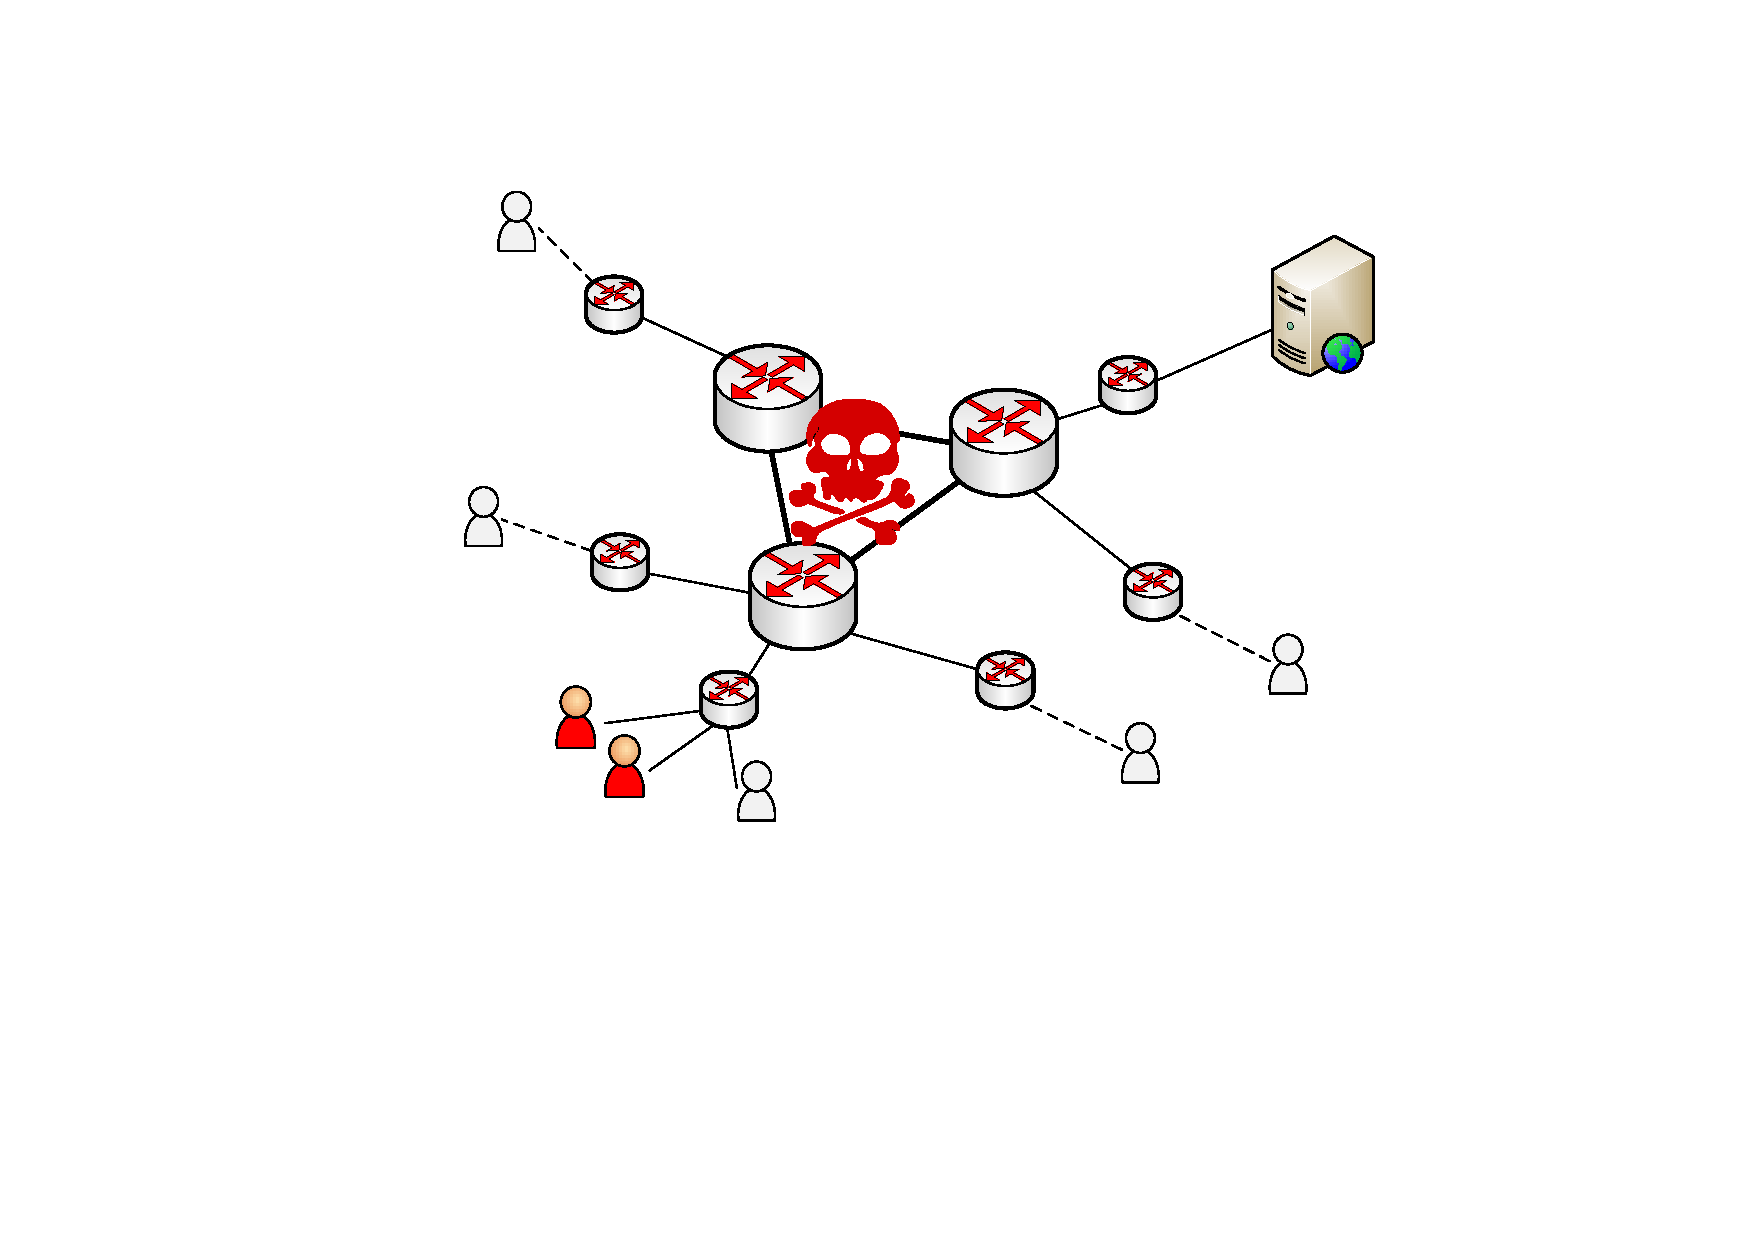
\includegraphics[scale=.3]{figures/scenario4-core-selective.pdf}
  \end{figure}
\begin{block}{Can be indistinguishable from non-selective attacks}
  \begin{itemize}
    \item \textit{Every} attack report to be checked for plausibility
    \item But attacker should leave some hints -- cannot arbitrarily spoof IP addresses
  \end{itemize}
\end{block}
\end{frame}



\begin{frame}
\frametitle{Patterns to look for}
\begin{block}{Attack seems to be restricted to few stub AS}
  \begin{itemize}
    \item Use BGP data to check traceroutes for plausibility
    \item Do MitM certificates share properties?
    \item Which AS in which countries involved?
  \end{itemize}
\end{block}
\begin{block}{MitM reports from just a few companies?}
  \begin{itemize}
    \item Check traceroutes for traversed countries and AS
    \item Might be industrial espionage
  \end{itemize}
\end{block}
\begin{block}{All of this is intensive manual work. But only localisation is affected, and it is better than no data all.}\end{block}
\end{frame}



\begin{frame}
\frametitle{Other issues}
\begin{block}{Crossbear is an open system}
\begin{itemize}
  \item Malicious injection of data
    \begin{itemize}
      \item Clients/hunters have no ID, no authentication
      \item Attacker can eclipse real hunters in his network, too
      \item Should results in clusters of suspicious reports, though
    \end{itemize}
  \item Denial-of-service attacks
  \item It is an arms race
  \item Other detection systems are subject to same attacks
\end{itemize}
\end{block}
\end{frame}
